\documentclass[a4paper, 10pt, final, garamond]{book}
\usepackage{cours-preambule}
\graphicspath{{./figures/}}

\makeatletter
\renewcommand{\@chapapp}{Contr\^ole de connaissances}
\makeatother

% \toggletrue{student}
% \HideSolutionstrue

\begin{document}
\setcounter{chapter}{1}

\chapter{Optique~: dispositifs optiques}

\ifstudent{
	\begin{tikzpicture}[remember picture, overlay]
		\node[anchor=north west, align=left] at (current page.north west)
		{\\[5pt]Nom~:\\[10pt]Prénom~:};
	\end{tikzpicture}
}

\begin{enumerate}[label=\sqenumi, leftmargin=10pt]
	\nitem{3} Démontrer la relation de conjugaison de \textsc{Newton}. Un schéma
	est attendu.
	\smallbreak
	\begin{isd}[righthand ratio=.3]
		\wsw{
			On utilise le théorème de \textsc{Thalès} dans les triangles F$'$OH et
			F$'$A$'$B$'$, en remarquant que $\obar{\rm OH} = \AB$, et les
			triangles FAB et FOH' pour avoir
			\begin{gather*}
				\frac{\obar{\rm A'B'}}{\obar{\rm OH}} = \frac{\ABp}{\AB} =
				\frac{\obar{\rm F'A'}}{\obar{\rm F'O}}
				\qqet
				\frac{\obar{\rm OH'}}{\obar{\rm AB}} = \frac{\ABp}{\AB} =
				\frac{\obar{\rm FO}}{\obar{\rm FA}}
				\\\Lra
				\boxed{\gamma = - \frac{\obar{\rm F'A'}}{\OFp}}
				\qqet
				\boxed{\gamma = - \frac{\OF}{\obar{\rm FA}}}
			\end{gather*}
			En les combinant on obtient
			\begin{empheq}[box=\fbox]{align*}
				\OFp\times\OF    & = \obar{\rm F'A'}\obar{\rm FA}\\
				\Leftrightarrow -f'^2 & = \obar{\rm F'A'}\obar{\rm FA}
			\end{empheq}
		}
		\vspace{-10pt}
		\tcblower
		\begin{center}
			\switch{
				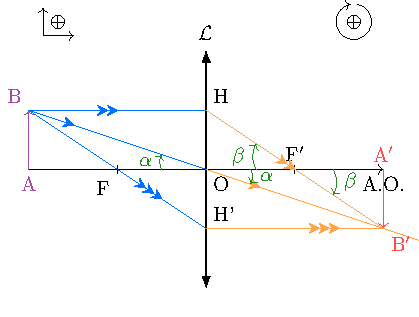
\includegraphics[width=\linewidth, draft=true]{lent_conv-demo}
			}{
				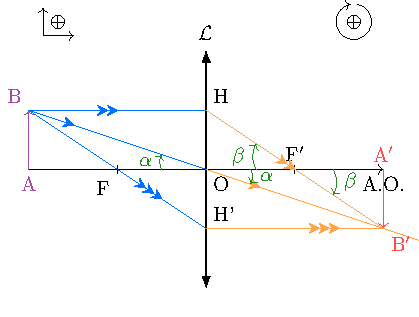
\includegraphics[width=\linewidth]{lent_conv-demo}
			}
			\captionof{figure}{Schéma}
			\label{fig:lent_rc}
		\end{center}
	\end{isd}

	\nitem{3}
	Quelles sont les valeurs maximale et minimale de la focale du cristallin
	pour un œil emmétrope~? On rappelle que la distance cristallin-rétine est $d
		\approx \SI{22.3}{mm}$. Un schéma est attendu pour la situation
	d'accomodation.
	\begin{isd}[righthand ratio=.3]
		\wsw{
			Pour le remotum on a directement que la focale doit être égale à la
			distance cristallin-rétine, puisqu'un objet à l'infini se forme dans le
			plan focal image. Pour le proximum, on utilise la relation de conjugaison
			avec A$'$ = E, $\OA = \SI{-25}{cm}$ et on trouve $f'$ :
			\begin{gather*}
				\xul{\OFp_\mathrm{repos} = \SI{22.3}{mm}}
				\text{, }
				\boxed{
					\OFp_{\rm acco} = \frac{\obar{\rm OE}\OA}{\OA - \obar{\rm OE}}
				}
				\\
				\mathrm{A.N.~:}\enskip
				\xul{
					\OFp_{\rm acco} = \SI{21}{mm}
				}
			\end{gather*}
		}
		\vspace*{-20pt}
		\tcblower
		\begin{center}
			\switch{
				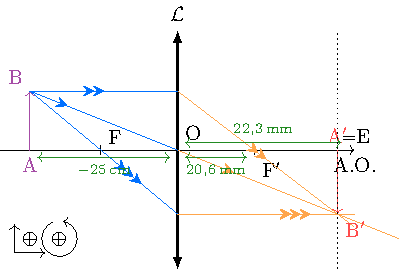
\includegraphics[width=\linewidth, draft=true]{oeil_acco}
			}{
				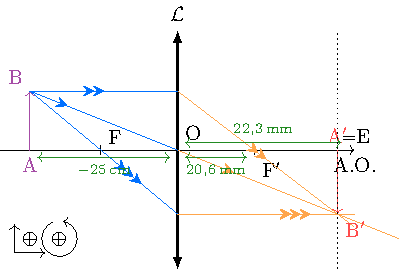
\includegraphics[width=\linewidth]{oeil_acco}
			}
			\captionof{figure}{Schéma}
		\end{center}
	\end{isd}
	\nitem{4} Deux lentilles minces convergentes $\Lc_1$ de centre optique O$_1$ et
	$\Lc_2$ de centre optique O$_2$ sont disposées selon le schéma ci-dessous.
	Trouver la position de l'image finale $\ABp$ de l'objet AB donnée par
	l'association $\Lc_1 + \Lc_2$, et donner la nature de tous les objets et
	images.
	\begin{center}
		\switch{
			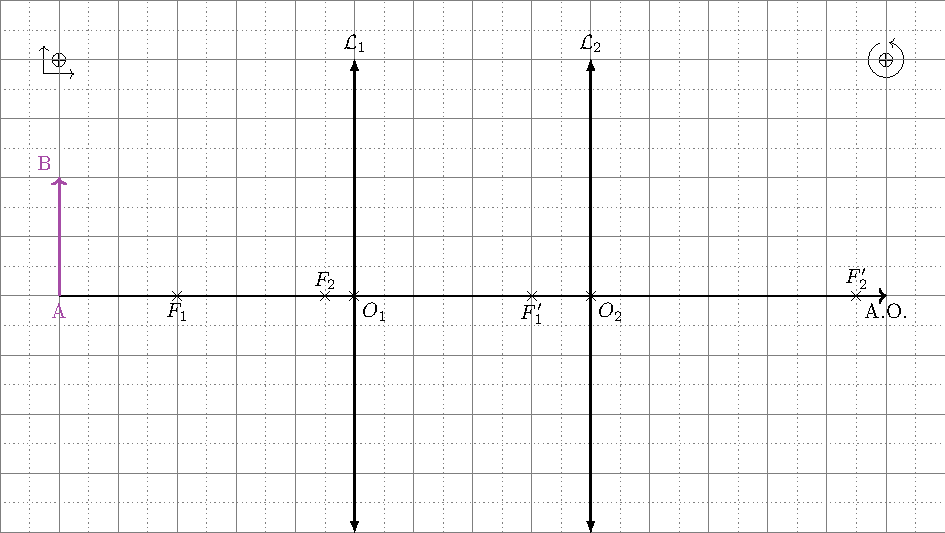
\includegraphics[width=.85\linewidth]{asso_lent-a_plain}
		}{
			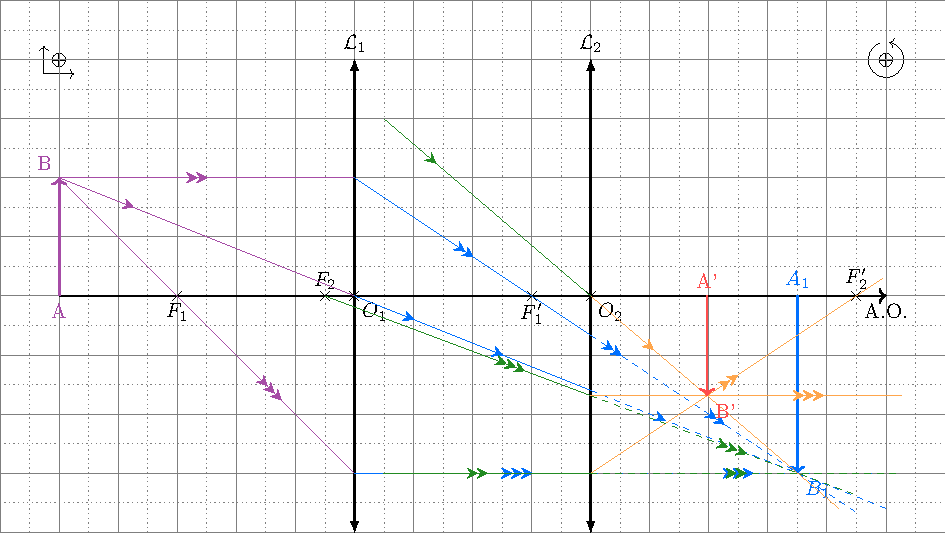
\includegraphics[width=.85\linewidth]{asso_lent-a}
		}
	\end{center}
\end{enumerate}
\end{document}
